
%%%%%%%%%%%%%%%%%%%%%%%%%%%%%%%%%%%%%%%%%%%%%%%%%%%%%%%%%%%%%%%%%%%%
%%%%%%%% Released for translation     10.4.2023 %%%%%%%%%%%%%%%%%%%%
%%%%%%%% Re-released for translation  22.6.2023 %%%%%%%%%%%%%%%%%%%%
%%%%%%%% Re-released for translation 26.12.2023 %%%%%%%%%%%%%%%%%%%%
%%%%%%%% Re-released for translation 04.01.2024 %%%%%%%%%%%%%%%%%%%%
%%%%%%%%%%%%%%%%%%%%%%%%%%%%%%%%%%%%%%%%%%%%%%%%%%%%%%%%%%%%%%%%%%%%

\noindent
\brcolor{\LARGE Prefacio}\label{primer-preface}\label{preface} 
\addcontentsline{toc}{section}{\brcolor{Prefacio}}
\minitoc
 
\begin{flushright}\label{front-Dogma}
\sort{El Dogma del Tríptico}\\[4mm]
\addcontentsline{toc}{subsection}{\bbcolor{El Dogma del Tríptico}}
\sf Para \textsl{especificar} \bmcolor{software},\\
\sf debemos entender sus requisitos.\\[1mm]
\sf Para \textsl{prescribir} \bmcolor{requisitos}\ysfchg{,}\\
\sf debemos entender el \bmcolor{dominio}.\\[1mm]
\sf Por lo tanto, debemos \bbcolor{estudiar, analizar} y \bbcolor{describir} los dominios.
\end{flushright}\rm%
\index{pdefind}{El Dogma del Tríptico}\index{pdefind}{Tríptico!Dogma, El}%\index{pdefind}{Dogma, El Tríptico}

\subsection*{\bbcolor{Dominios -- ¿Qué Son?}}
\addcontentsline{toc}{subsection}{\bbcolor{Dominios -- ¿Qué Son?}}

\pos{\normalsize}{\HHHH}


\label{1stdd}
\ysf{\domaindefinition}
\pos{\psno}{\mnewfoil}

\renewcommand{\newdbsquare}{\dbsquare}

\begynd
\pind \sort{Ejemplos} \ysfchg{d}e dominios son:
\begynd
\pind {\sl transporte ferroviario, por carretera, marítimo y aéreo;
\pind tuberías de agua, petróleo y gas;
\pind manufactura industrial;
\pind la industria de servicios financieros: clientes, bancos, tarjetas de crédito, acciones, etc.;
\pind mercados de consumo, minorista y mayorista;
\pind atención médica;}
\pind etcétera.
\afslut
\afslut
\subsection*{\bbcolor{Meta y Objetivos}}\addcontentsline{toc}{subsection}{\bbcolor{Meta y Objetivos}}  

\vspace*{-4mm}

\begin{itemize}
\item La \sort{meta} de esta \monograph es contribuir a una 
      metodología para analizar y describir dominios.
  
\item Los \sort{objetivos} -- en el sentido de `cómo se logra la meta' -- se reflejan en la estructura y el contenido
      y el enfoque didáctico de esta \monograph.
\item Los elementos principales de \ysfchg{nuestro} enfoque -- a lo largo de un
  eje conceptual -- se pueden enumerar: 
\begin{itemize}
\item Está el fundamento de nuestro enfoque de análisis y descripción
      en proporcionar una base \sort{filosófica},
      cf.\,capítulo\,\ref{chap2.tex.Philosophy}. 
\item Está la aplicación de ideas de \sort{taxonomía} 
      para entender la estructuración posiblemente jerárquica
      de los fenómenos del dominio, logrando una comprensión de las propiedades
      de los fenómenos y las relaciones entre ellos.
\item Están las nociones de \sort{endurantes} y \sort{perdurantes} -- % After giving it some thought, I think I align with "making up" the endurante and perdurante terms and just addding a footnore clariying what they mean.
      con los \sfsl{endurantes}  \index{pdefind}{endurante} siendo los fenómenos
\begynd
\pind que pueden ser observados, o concebidos y descritos, como \nyl una ``cosa completa'' en cualquier instante dado de tiempo\pos{
      \cite[vol.\,I, pág.\,656]{OED}}{},
\afslut
      y los \sfsl{perdurantes}  \index{pdefind}{perdurante} siendo los fenómenos 
\begynd
\pind de los cuales solo existe un fragmento\pos{}{\\} si los observamos o
      los tocamos\pos{}{\\} en cualquier instante dado de tiempo\pos{
      \cite[vol.\,II, pág.\,1552]{OED}}{}.
\afslut
\item Está la introducción de elementos base de
      \sort{cálculos}  \index{pdefind}{cálculos} para analizar y
      describir dominios. \index{pdefind}{cálculo!análisis}
\item Está la aplicación de ideas de \sort{ontología} 
      para entender la estructuración posiblemente jerárquica
      de estos cálculos.\index{pdefind}{ontología} 
\item Finalmente, está la noción de la
      \index{pdefind}{deducción trascendental} \sort{deducción
      trascendental}, cf.\,Sect.\,\ref{sec:Transcendence}, para ``transformar''
      ciertos tipos de endurantes en ciertos tipos de perdurantes,
      capítulo \ref{chap6.tex.1}.
\end{itemize}
\item A lo largo de otro eje conceptual, tenemos los siguientes elementos adicionales
        de nuestro enfoque:
\begin{itemize}
\item Consideramos que las descripciones de dominio, las prescripciones de requisitos y
      las especificaciones de diseño de software son cantidades \brcolor{matemáticas}
      \index{pdefind}{matemáticas}.
\item Las consideramos básicamente en el sentido de la
      \sort{teoría de funciones recursivas}
      \index{pdefind}{teoría de funciones recursivas} \cite[Hartley Rogers,
      1952]{Rogers67} y  la
      \sort{teoría de tipos}  \index{pdefind}{teoría de tipos} \cite[Benjamin
      Pierce, 1997]{pierce1997}.  
\end{itemize}
\end{itemize}

\vspace*{-4mm}
\subsection*{\bbcolor{Metodología}}\addcontentsline{toc}{subsection}{\bbcolor{Metodología}}\label{front:Methodology}

\begynd
\pind Por \sort{método} entenderemos
\begynd
\pind un conjunto de \sort{principios}\index{pdefind}{principio}
\footnote{Por \sort{principio} nos referimos a:
  \sfsl{un principio es una proposición o valor que sirve como guía para
    el comportamiento o la evaluación \wiki, es decir, un código de conducta}}
y \sort{procedimientos}\index{pdefind}{procedimiento}%
\footnote{Por 
  \sort{procedimiento} nos referimos a: \sfsl{instrucciones o recetas, un conjunto de comandos
    que muestran cómo lograr algún resultado, como preparar o hacer
    algo \wiki, es decir, una forma establecida de hacer algo}} 
\pind para seleccionar y aplicar un conjunto de
\sort{técnicas}\index{pdefind}{técnica}%
\footnote{Por \sort{técnica} nos referimos a: \sfsl{una técnica, o destreza, es
    la capacidad aprendida para realizar una acción con resultados determinados
    con buena ejecución, a menudo dentro de una cantidad de tiempo y energía
    dada, o ambas \wiki, es decir, una manera de
    llevar a cabo una tarea particular}}
y \sort{herramientas}\index{pdefind}{herramienta}%
\footnote{Por 
  \sort{herramienta} nos referimos a: \sfsl{una herramienta es un objeto que puede extender la
    capacidad de un individuo para modificar características del entorno
    circundante \wiki}} a un problema  
\afslut
\pind para lograr una construcción ordenada de una
      \sort{solución}, es decir, un \sort{artefacto}.
\afslut
\mnewfoil
\begynd
\pind Por \sort{metodología} entenderemos
\begynd
\pind el \sfsl{estudio \& aplicación} de uno o más métodos.
\afslut
\afslut
\mnewfoil

\pind Por \sort{método formal} entenderemos un método:
\begin{itemize}
\item cuyos \sfsl{principios} incluyen considerar sus artefactos como % I don't understand the original meaning of this paragraph
      cantidades \sfsl{matemáticas}, como \sfsl{abstracciones}, etc.
\item cuyos \sfsl{procedimientos} decisivos incluyen:
\begin{itemize}
\item el análisis
      \ysfchg{\&} descripción secuencial primero de los endurantes, seguido por los perdurantes
\item dentro del análisis \ysfchg{\&} descripción de los endurantes,
      el análisis \ysfchg{\&} descripción secuencial primero de sus cualidades externas y luego de sus cualidades internas
\item etc.
\end{itemize}
\item cuyas \sfsl{técnicas} incluyen formas específicas de
       especificar propiedades
\item cuyas \sfsl{herramientas} incluyen uno o más
      \sort{lenguajes formales} % Needs revision for conjunctions and punctuation :/
\end{itemize}
\mnewfoil

\noindent
\begynd
\pind Por \sort{lenguaje} entenderemos aquí \nyl un conjunto de
cadenas de caracteres, es decir, oraciones,
\begynd
\pind oraciones que están estructuradas según alguna \sort{sintaxis},
      es decir, \sort{gramática},
\pind a las que se les da significado por alguna \sort{semántica},
\pind y que se utilizan según alguna \sort{pragmática}. 
\afslut
\afslut

\begynd
\pind Por \sort{lenguaje formal} entenderemos aquí un lenguaje
\begynd
\pind cuya \sfsl{sintaxis} y \sfsl{semántica} pueden ser expresadas
      \sort{matemáticamente}
\pind y para cuyas oraciones se puede \sort{razonar racionalmente} % Unsure where we want an "and" here or if "probar propiedades" is the intended meaning.
      (\sfsl{argumentar, probar}) \sort{propiedades}. 
\afslut

\pind Nos referimos al capítulo\,1 de \cite{BjornerMonograph2020} para un conjunto de
      definiciones de conceptos de 8 páginas y aproximadamente 50 entradas como las anteriores.
      
\pind Nos referimos al índice de \textsf{Método}, sect.\,\vref{label.dadmethod}.
\afslut
      
\treprikker

\noindent
\pind En este \primer usaremos
\begynd 
\pind el lenguaje de especificación formal, \texttt{RSL},
\pind el \texttt{R}AISE\footnote{\sort{RAISE: "R}igorous
      \sort{A}pproach \ysfchgii{ }
      to \ysfchg{\sort{I}ndustrial } \sort{S}oftware \sort{E}ngineering" (enfoque riguroso de la ingeniería industrial), % This is hard to translate for me. 
      \cite{RaiseMethod}} \texttt{S}pecification 
      \texttt{L}anguage, \cite{RSL} -- 
\pind y nos basaremos notablemente en la adaptación de \texttt{RSL} de \sort{CSP}, los
      \sfsl{Procesos Secuenciales Comunicantes ("Communicating Sequential Processes")} de Tony Hoare \citecsp;
\pind y propagaremos un método definitivo para el estudio y
      descripción de dominios.
\afslut
\afslut

\subsection*{\bbcolor{Un Énfasis}}\addcontentsline{toc}{subsection}{\bbcolor{Un Énfasis}} 

\anemphasis{Los dominios exhiben endurantes y perdurantes. Un modelo de dominio
  es, por lo tanto, algo que define los \sfsl{sustantivos} (hablando en términos generales, los
  endurantes) y los \sfsl{verbos} (hablando en términos generales, los {perdurantes}) -- y
  su combinación -- de un
  \sfsl{lenguaje} hablado y usado por escrito por los practicantes del dominio. No es una
  instanciación de sustantivos, verbos y su combinación,
  sino todas las posibles y sensatas instanciaciones.}{}

\subsection*{\bbcolor{Una Advertencia}}\addcontentsline{toc}{subsection}{\bbcolor{Una Advertencia}}

Los lectores experimentados de \texttt{RSL} \cite{RSL} podrían observar nuestro,
quizás despreocupado (informal), uso de \texttt{RSL}. Quizás, en algunos lugares, la 
sintaxis de las cláusulas de \texttt{RSL} no sea del todo correcta. Nuestro no uso
de los constructos de módulos (\texttt{Esquema}\ysfchg{, } \texttt{Clase} y \texttt{Objeto})
de \texttt{RSL} \ysfchg{nos} fuerza a declarar \textsf{canal}es de la misma manera
en que se introducen \textsf{tipo}s, \textsf{valor}es y \textsf{variable}s.

\begin{itemize}
%%\item[] \hfill 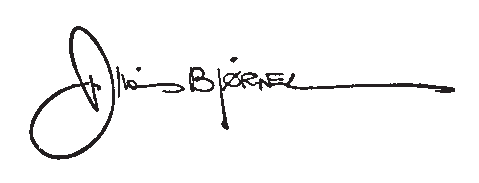
\epsfig{file=db.eps,height=25mm}

%%\vspace*{-12mm}
\item[] \hfill   Dines Bj{\o}rner \& Yang ShaoFa

\item[] \hfill \todaytime
\end{itemize}


\label{preface.n}
%%  LocalWords:  analyse defind artefactual et cetera analysing RSL
%%  LocalWords:  endurants perdurants endurant perdurant Hartley AISE
%%  LocalWords:  pdefind artefact artefacts dadmethod igorous pproach
%%  LocalWords:  oftware ngineering pecification anguage CSP Hoare's
%%  LocalWords:  instantiation instantiations ndustrial Bj rner
%%  LocalWords:  ShaoFa
